\documentclass[11pt]{article}
\usepackage[margin=1in]{geometry}
\usepackage{amsmath,amssymb,amsthm,mathtools}
\usepackage{booktabs}
\usepackage{array}
\usepackage{xcolor}
\usepackage{enumitem}
\usepackage{tikz}
\usetikzlibrary{patterns,arrows.meta,decorations.pathreplacing}
\usepackage[hidelinks]{hyperref}
\usepackage{microtype}

\theoremstyle{plain}
\newtheorem{theorem}{Theorem}[section]
\newtheorem{proposition}[theorem]{Proposition}
\newtheorem{lemma}[theorem]{Lemma}
\newtheorem{corollary}[theorem]{Corollary}
\theoremstyle{definition}
\newtheorem{definition}[theorem]{Definition}
\theoremstyle{remark}
\newtheorem{remark}[theorem]{Remark}

\definecolor{forcedc}{RGB}{15,110,86}
\definecolor{declaredc}{RGB}{24,95,165}
\definecolor{positedc}{RGB}{170,105,20}
\definecolor{openc}{RGB}{163,45,45}
\definecolor{boxfill}{RGB}{226,240,234}
\definecolor{forbidfill}{RGB}{248,228,228}
\newcommand{\forced}{\textcolor{forcedc}{\textsc{[forced]}}}
\newcommand{\declared}{\textcolor{declaredc}{\textsc{[declared]}}}
\newcommand{\posited}{\textcolor{positedc}{\textsc{[posited]}}}
\newcommand{\openq}{\textcolor{openc}{\textsc{[open]}}}
\newcommand{\computed}{\textcolor{forcedc}{\textsc{[computed]}}}

\newcommand{\R}{\mathbb{R}}
\newcommand{\Q}{\mathbb{Q}}
\newcommand{\Z}{\mathbb{Z}}
\newcommand{\Cx}{\mathbb{C}}
\newcommand{\T}{\mathbb{T}}
\newcommand{\D}{\mathbb{D}}
\newcommand{\tr}{\operatorname{tr}}
\newcommand{\Mah}{\mathrm{M}}
\newcommand{\spec}{\operatorname{spec}}
\newcommand{\charp}{\chi}
\newcommand{\argc}{\operatorname{Arg}_{\partial}}
\newcommand{\norm}[1]{\left\lVert #1 \right\rVert}
\newcommand{\abs}[1]{\left\lvert #1 \right\rvert}
\newcommand{\Scal}{\mathcal{S}}
\newcommand{\Acal}{\mathcal{A}}
\newcommand{\Ccal}{\mathcal{C}}
\renewcommand{\Box}{\mathfrak{B}}
\newcommand{\ad}{\operatorname{ad}}

\title{\textbf{Lehmer's Box:}\\[2pt]
\large A Golden Floor and an Angle Lattice that Confine Spectral Emission\\
Away from Salem Numbers --- Without Resolving Lehmer's Problem\\[6pt]
\normalsize A Companion to \emph{The Emission--Gap Theorem} and \emph{The Exchange Rate $\lambda=2c$}}
\author{Echo--Squirrel Research}
\date{}

\begin{document}
\maketitle

\begin{abstract}
The residual--return growth rule charges $\lambda\log\Mah(\theta)$ to adjoin an algebraic direction $\theta$, where $\Mah$ is the Mahler measure. The rule has a strictly positive cost floor exactly when $\Mah$ is bounded away from $1$ over every spectrum the construction can emit. The single obstruction is the Salem number: a reciprocal unit with conjugates on the unit circle, evading Smyth's non--reciprocal bound $\Mah\ge\mu_S$, and able --- as far as anyone has proved in ninety years --- to lie arbitrarily close to $1$. Deciding whether Salem numbers approach $1$ is \emph{Lehmer's problem}, open since 1933. We do not resolve it. We build a box around it.

This paper formulates, from first principles, the geometric object that the Emission--Gap Theorem implicitly constructs: \emph{Lehmer's Box}, the region of height--angle space cut out by two walls. The \emph{floor wall} is the golden value $\varphi$: the open Mahler strip $(1,\varphi)$ is empty for integer quadratics, and the spectral operators preserve that emptiness, so every emitted measure lies in $\{1\}\cup[\varphi,\infty)$. The \emph{lattice walls} are the four directions $\tfrac{\pi}{2}\Z$: every catalog eigenvalue has argument in $\tfrac{\pi}{2}\Z$, the operators are closed under angle--addition and angle--doubling but not halving, so every emitted on--circle eigenvalue is a fourth root of unity. A Salem number violates both walls at once --- its on--circle conjugates carry irrational angle (off the lattice) and its measure may sit below $\varphi$ (under the floor). The box and the Salem locus are therefore disjoint; the spectral image omits every Salem number, and with it the whole band $(1,\mu_S)$.

We give the box four faces --- height, angle, field signature, and trace--down flip --- and show they are one object seen from four sides; the signature face confines the only place a real Salem could graze the floor to the Lorentzian quartic $\Q(5^{1/4})$, where the minimal degree--four Salem $\beta_4=1.7221\ldots>\varphi$ keeps the floor intact. The box has exactly one door: the free commutator, which by Shoda's theorem can carry any traceless matrix, including a foreign sub--$\varphi$ Salem. We close that door two ways: structurally, by identifying the framework's commutator as the self--action $\ad_R=[R,\cdot]$, a derivation whose spectrum is forced into the difference field $K=\Q(\sqrt2,\sqrt3,5^{1/4})$; and operationally, by an exact runtime lock that decides $\beta<\varphi$ by the sign of an element of $\Q(\sqrt5)$ with no floating point. Finally we state the logic of the sidestep precisely: the box theorem is unconditional within the system, strictly weaker than Lehmer's conjecture, and consistent with both truth values of Lehmer --- it routes around the open problem rather than settling it. Every non--asymptotic claim is machine--verified in exact arithmetic; the backing test identifiers are named inline.
\end{abstract}

\tableofcontents

\section{Introduction: the floor, the obstruction, and the box}\label{sec:intro}

\subsection{Why a floor is needed}
The construction we analyse grows an exact symbolic state by occasionally adjoining a new algebraic direction $\theta$. The price charged for that adjunction is
\begin{equation}\label{eq:cost}
\text{cost}(\theta)\ =\ \lambda\,\log\Mah(\theta),
\end{equation}
where $\Mah$ is the Mahler measure (Section~\ref{sec:mahler}) and $\lambda=2c$ is the derived exchange rate of the companion paper. For \eqref{eq:cost} to be a usable description length --- for growth to be genuinely \emph{paid for} rather than free --- the price of any non--trivial adjunction must be bounded below by a fixed positive amount:
\begin{equation}\label{eq:floorgoal}
\inf\bigl\{\,\Mah(\theta):\theta\ \text{emittable},\ \Mah(\theta)>1\,\bigr\}\ >\ 1.
\end{equation}
Equation \eqref{eq:floorgoal} is the entire question this paper answers --- but only for the directions the construction can actually emit, and that restriction is the whole point.

\subsection{The obstruction is a single, named, open problem}\label{sec:obstruction}
The infimum in \eqref{eq:floorgoal}, taken over \emph{all} integer polynomials rather than only emittable ones, is the subject of a ninety--year--old open problem. Two classical facts bracket it. By Kronecker's theorem (Section~\ref{sec:mahler}), $\Mah(p)=1$ holds exactly for the cyclotomic polynomials --- the trivial floor. By Smyth's theorem \cite{Smyth}, every \emph{non--reciprocal} monic integer polynomial satisfies
\[
\Mah(p)\ \ge\ \mu_S\ =\ 1.3247179572\ldots,
\]
the plastic number, the real root of $x^3-x-1$ and the smallest Pisot number. The only way to approach $1$ from above is therefore through \emph{reciprocal} polynomials --- and among these, the \emph{Salem numbers}. The smallest measure ever exhibited, Lehmer's number
\[
\Mah(L)\ =\ 1.1762808182\ldots\qquad
L(x)=x^{10}+x^9-x^7-x^6-x^5-x^4-x^3+x+1,
\]
is a Salem number, and it already lies below $\mu_S$. Whether Salem numbers are bounded away from $1$ at all is \textbf{Lehmer's problem} \cite{Lehmer}, open since 1933; Dobrowolski's bound $\Mah(p)>1+c\,(\log\log n/\log n)^3$ \cite{Dobrowolski} decays to $1$ with the degree $n$ and so yields no uniform floor. We will not move this problem. We will make it irrelevant to \eqref{eq:floorgoal}.

\subsection{The thesis: confinement, not resolution}\label{sec:thesis}
The strategy is a single structural implication. Suppose one can show that the construction's emission image avoids every Salem number. Then it avoids the entire band $(1,\mu_S)$ --- because every measure in that band is realised only by a reciprocal Salem--type number, non--reciprocals being bounded below by $\mu_S$ via Smyth. Smyth's bound then supplies \eqref{eq:floorgoal} with floor $\mu_S$, and the realised stock attains the sharper value $\varphi=1.6180339887\ldots$. Crucially, this never touches Lehmer, because ``no Salem in the image'' is a \emph{closure property of one specific algebra}, not a universal height bound.

This paper packages that closure as a geometric object. We introduce \emph{Lehmer's Box} (Definition~\ref{def:box}): the set of monic integer polynomials whose Mahler measure avoids the strip $(1,\varphi)$ (the \emph{floor wall}) and whose on--circle roots all sit at the four lattice directions $\tfrac{\pi}{2}\Z$ (the \emph{lattice walls}). The two central theorems are then short to state:
\begin{itemize}[leftmargin=1.4em]
\item \textbf{Emission $\subseteq$ Box} (Theorem~\ref{thm:emitbox}): every spectrum the construction emits lies in $\Box$.
\item \textbf{Salem $\cap$ Box $=\varnothing$} (Theorem~\ref{thm:salemoutside}): no Salem number's minimal polynomial lies in $\Box$.
\end{itemize}
Their conjunction is the exclusion: the emission image contains no Salem number, the cost floor of \eqref{eq:floorgoal} is positive (Corollary~\ref{cor:floor}), and Lehmer's number --- still a perfectly good number --- is simply \emph{not in the box}, hence never emitted. Section~\ref{sec:sidestep} states the precise logical relationship between the box theorem and Lehmer's problem: the former is unconditional, strictly weaker than the latter, and consistent with either of its truth values. That triple is what we mean by \emph{sidestepping Lehmer without disproving it}.

\subsection{Roadmap}
Section~\ref{sec:prelim} fixes the Mahler measure, Kronecker, the Salem/Pisot vocabulary, and the catalog and operators from scratch. Section~\ref{sec:floor} derives the floor wall (the empty strip $(1,\varphi)$ and its preservation under the operators). Section~\ref{sec:walls} derives the lattice walls (the four angle lemmas). Section~\ref{sec:box} defines Lehmer's Box and proves the two central theorems and the floor corollary. Sections~\ref{sec:sigface}--\ref{sec:flipface} give the field--signature and trace--down faces of the same box. Section~\ref{sec:door} treats the one door --- the free commutator --- structurally (the self--action derivation) and operationally (the exact guard). Section~\ref{sec:sidestep} is the logic of the sidestep. Section~\ref{sec:ledger} is the epistemic ledger keyed to the machine--verified tests.

\section{Preliminaries, from scratch}\label{sec:prelim}

\subsection{The Mahler measure}\label{sec:mahler}
\begin{definition}[Mahler measure]\label{def:mahler}
For a nonzero $p(x)=a_d\prod_{i=1}^d(x-\alpha_i)\in\Z[x]$ with $a_d\neq0$,
\begin{equation}\label{eq:mahdef}
\Mah(p)\ =\ \abs{a_d}\prod_{i=1}^{d}\max\!\bigl(1,\abs{\alpha_i}\bigr)
\ =\ \exp\!\left(\int_0^1\log\bigl|p(e^{2\pi i\theta})\bigr|\,d\theta\right).
\end{equation}
The two expressions agree by Jensen's formula. For an algebraic number $\theta$ we write $\Mah(\theta):=\Mah(m_\theta)$, the measure of its monic integer minimal polynomial.
\end{definition}

The product form makes the basic inequality immediate.

\begin{lemma}[Lower bound and its multiplicativity]\label{lem:mahbasic}
For monic $p,q\in\Z[x]$: \emph{(i)} $\Mah(p)\ge1$; \emph{(ii)} $\Mah(pq)=\Mah(p)\Mah(q)$; \emph{(iii)} if $p^{[2]}$ denotes the polynomial whose roots are the squares of those of $p$, then $\Mah(p^{[2]})=\Mah(p)^2$.
\end{lemma}
\begin{proof}
(i) Each factor $\max(1,\abs{\alpha_i})\ge1$ and $\abs{a_d}=1$. (ii) The root multiset of $pq$ is the union, and $\max(1,\cdot)$ is multiplicative across a union of factors. (iii) $\max(1,\abs{\alpha}^2)=\max(1,\abs{\alpha})^2$, taken over the same roots.
\end{proof}

The boundary case $\Mah=1$ is settled completely and classically.

\begin{lemma}[Kronecker, 1857]\label{lem:kronecker}
A monic $p\in\Z[x]$ has all roots in the closed unit disk if and only if every root is $0$ or a root of unity. Consequently $\Mah(p)=1$ iff $p(x)=x^{k}\prod_j\Phi_{n_j}(x)$ is a power of $x$ times cyclotomic factors.
\end{lemma}
\begin{proof}[Proof sketch]
If a nonzero monic integer $p$ has all roots in $\overline{\D}$, then so do all its powers under the maps $\alpha\mapsto\alpha^{m}$; the elementary symmetric functions of $\{\alpha_i^m\}$ are bounded integers, so the polynomials $p_m(x)=\prod_i(x-\alpha_i^m)$ range over a finite set as $m$ varies. By pigeonhole two coincide, forcing the multiset $\{\alpha_i\}$ to be permuted by some power map; a root fixed by $\alpha\mapsto\alpha^{m}$ with $\abs\alpha\le1$ and $\alpha\neq0$ has $\abs\alpha=1$ and is a root of unity. The converse is immediate since roots of unity and $0$ lie in $\overline\D$.
\end{proof}

\subsection{Pisot, Salem, and Smyth}\label{sec:salemvocab}
\begin{definition}[Pisot and Salem numbers]\label{def:pisotsalem}
A \textbf{Pisot number} is a real algebraic integer $\beta>1$ all of whose other conjugates lie strictly inside the unit circle. A \textbf{Salem number} is a real algebraic integer $\beta>1$ all of whose conjugates lie in the closed unit disk, with at least one on the unit circle. Equivalently, $m_\beta$ is reciprocal of even degree $2m\ge4$, with real roots $\beta,\beta^{-1}$ and $m-1$ conjugate pairs on $\abs z=1$. The \textbf{Salem band} is the interval $(1,\mu_S)$.
\end{definition}

A polynomial $p$ is \textbf{reciprocal} if its root multiset is closed under $\alpha\mapsto\alpha^{-1}$, equivalently $x^{\deg p}p(1/x)=p(x)$; otherwise \textbf{non--reciprocal}. Salem minimal polynomials are reciprocal. The asymmetry that the whole construction exploits is Smyth's:

\begin{lemma}[Smyth's bound]\label{lem:smyth}
Every non--reciprocal monic integer polynomial with $\Mah>1$ satisfies $\Mah(p)\ge\mu_S=1.3247\ldots$, the smallest Pisot number \cite{Smyth}.
\end{lemma}

Smyth closes the non--reciprocal side of \eqref{eq:floorgoal} outright. Everything difficult lives on the reciprocal side, and concretely in the Salem band, where Lehmer's number already sits.

\subsection{The catalog and the operators}\label{sec:catalog}
The construction emits matrices from a finite catalog of seed companions under a fixed operator set. We restate both from the companion paper.

\begin{definition}[Catalog]\label{def:catalog}
$\Ccal=\{C(m_\theta):\theta\in\{\varphi,\tau,\sqrt2,\sqrt3,\sqrt5,\mathrm{gap},K\}\}$, the companion matrices of, respectively,
\[
x^2-x-1,\quad x^2+x-1,\quad x^2-2,\quad x^2-3,\quad x^2-5,\quad x^2-7x+1,\quad x^4+5x^2-5 .
\]
Here $\varphi=\tfrac{1+\sqrt5}2$, $\tau=\tfrac{-1+\sqrt5}2=\varphi^{-1}$, $\mathrm{gap}=\varphi^4$ (roots $\varphi^{4},\varphi^{-4}$), and $K$ is the real root $5^{1/4}/\varphi$ of $x^4+5x^2-5$, whose four roots are $\{\pm K,\pm i\beta\}$ with $\beta\in\R$.
\end{definition}

\begin{definition}[Operators]\label{def:ops}
The \emph{spectral operators} determine the output spectrum from the input spectra:
\[
\oplus\ (\text{direct sum}),\quad \otimes\ (\text{tensor / Kronecker}),\quad (\cdot)^2\ (\text{squaring}),\quad \text{minpoly},\quad \Phi\ (\text{re--companion of the radical}).
\]
The \emph{entry--level operators} act on matrix entries and do \emph{not} determine the output spectrum from the inputs: the commutator $[A,B]=AB-BA$, the Cartan embeddings $A_n,D_n,E_8$, and the circulant $\operatorname{circ}(\cdot)$.
\end{definition}

\begin{definition}[Sub--algebra, image]\label{def:image}
$\Scal$ is the \emph{spectral emission algebra}: the closure of $\Ccal$ under the spectral operators. Its \emph{image} is the set of all eigenvalues of all matrices in $\Scal$, and $\Mah(\Scal)$ is the set of their Mahler measures. The full algebra $\Acal\supseteq\Scal$ additionally admits the entry--level operators.
\end{definition}

The reader should hold one picture: $\Scal$ is what the construction can build using only operations whose effect on the spectrum is forced by the inputs. The box is a statement about $\Scal$; the entry--level operators (Section~\ref{sec:door}) are the part that needs separate care.

\section{The floor wall: the empty strip \texorpdfstring{$(1,\varphi)$}{(1,phi)}}\label{sec:floor}

The first wall of the box is a lower fence on the height axis. We prove it at degree two, then show the spectral operators cannot tunnel under it.

\subsection{Base case: no integer quadratic measure between \texorpdfstring{$1$}{1} and \texorpdfstring{$\varphi$}{phi}}
\begin{lemma}[Empty quadratic strip]\label{lem:base}
No monic integer polynomial of degree $2$ has Mahler measure in the open interval $(1,\varphi)$. The measure is exactly $1$ on the cyclotomic quadratics and $\ge\varphi$ otherwise, with $\varphi$ attained only by $x^2-x-1$ and $x^2+x-1$ (discriminant $5$). \forced{} {\small(\texttt{P1-GATE-02}, \texttt{P1-GATE-03})}
\end{lemma}
\begin{proof}
Let $p=x^2+bx+c\in\Z[x]$ be irreducible and non--cyclotomic, so $\Mah(p)>1$ by Lemma~\ref{lem:kronecker}. Write the roots as $\alpha,\alpha'$ with $\alpha\alpha'=c$ and $\alpha+\alpha'=-b$.

\emph{Case $c=-1$ (reciprocal, hyperbolic).} The roots are real with product $-1$, so one lies outside and one inside the unit circle and $\Mah(p)=\abs\alpha$ where $\abs\alpha=\tfrac{\abs b+\sqrt{b^2+4}}2$. This is increasing in $\abs b$; its minimum over $\abs b\ge1$ is at $\abs b=1$, giving $\Mah=\tfrac{1+\sqrt5}2=\varphi$, realised by $x^2-x-1$ and $x^2+x-1$.

\emph{Case $c=1$ (reciprocal, elliptic/hyperbolic).} The roots form a reciprocal pair $\alpha,\alpha^{-1}$. For $\abs b\le1$ they lie on the unit circle and $p$ is cyclotomic ($x^2\pm x+1,\ x^2+1$), excluded. For $\abs b=2$, $p=(x\pm1)^2$ is reducible, excluded. For $\abs b\ge3$ the dominant root is $\tfrac{\abs b+\sqrt{b^2-4}}2\ge\tfrac{3+\sqrt5}2=\varphi^2$, so $\Mah\ge\varphi^2>\varphi$.

\emph{Case $\abs c\ge2$ (non--reciprocal).} If the roots are complex they are conjugate with $\abs\alpha=\sqrt{\abs c}\ge\sqrt2>1$, so $\Mah=\abs c\ge2$. If real, their product has absolute value $\abs c\ge2$, so the outside root contributes $\Mah\ge\abs c\ge2$ (a root inside the disk only raises the outside one).

In every case $\Mah(p)\ge\varphi$, with equality only at discriminant $5$. The interval $(1,\varphi)$ is thus unrealised; an exhaustive scan of all $625$ quadratics with $\abs b,\abs c\le12$ confirms both the empty interval and the minimiser.
\end{proof}

\subsection{Degree raising stays above the floor}
\begin{lemma}[The operators preserve the floor]\label{lem:degraise}
Under the spectral operators the Mahler image stays in $\{1\}\cup[\mu_S,\infty)$, with every realised value in $\{1\}\cup[\varphi,\infty)$. Hence $\Mah(\Scal)\subseteq\{1\}\cup[\mu_S,\infty)$, realised at $\varphi$. \forced{} {\small(\texttt{P2-GAP-02} ledger; \texttt{P2-EALG-01}, \texttt{P2-EALG-02})}
\end{lemma}
\begin{proof}
By Lemma~\ref{lem:mahbasic}(ii), $\Mah(p\oplus q)=\Mah(p)\Mah(q)$, and the product of two numbers in $\{1\}\cup[\varphi,\infty)$ stays there. By Lemma~\ref{lem:mahbasic}(iii), squaring squares the measure, so a value $>1$ maps to $\ge\varphi^2$. For $\otimes$ the spectrum is $\{\lambda_i\mu_j\}$; a factor is either Salem --- forbidden by Theorem~\ref{thm:salemoutside}, proved independently in Section~\ref{sec:box} --- or non--reciprocal with $\Mah\ge\mu_S$ by Smyth, or reciprocal non--Salem, which by Lemma~\ref{lem:salemirr} has all conjugates off the circle, hence is a real reciprocal unit with $\Mah\ge\varphi^2$. The operators $\text{minpoly}$ and $\Phi$ act on the same spectrum (radical, re--companion) and fix $\Mah$. Induction on word length from Lemma~\ref{lem:base} gives the image bound, with realised minimum $\varphi$ (the golden seed) and no realised value in $(1,\varphi)$.
\end{proof}

\begin{remark}[The image is a discrete semigroup]\label{rem:semigroup}
$\Scal$ is a finitely generated algebraic orbit; its Mahler spectrum is a discrete sub--semigroup of $[\varphi,\infty)$ generated by $\{\varphi,2,3,5,\varphi^4,\beta^2\}$ under multiplication ($\oplus$), squaring, and composition ($\otimes$), \emph{with no accumulation at $1$}. Limits are not operations: the construction cannot reach the Salem limit points of its own Pisot generators \cite{Salem}. This is an independent witness for the floor, consistent with the angle proof. \forced{} {\small(\texttt{P2-NL-04})}
\end{remark}

\section{The lattice walls: the four directions \texorpdfstring{$\tfrac{\pi}{2}\Z$}{(pi/2)Z}}\label{sec:walls}

The second wall is angular. The catalog sits at the four cardinal directions on the unit circle, the operators cannot manufacture a new direction, and a Salem number's on--circle conjugates refuse to sit at any of the four.

\begin{lemma}[Catalog arguments]\label{lem:catargs}
Every eigenvalue of every catalog matrix has argument in $\tfrac{\pi}{2}\Z=\{0,\tfrac\pi2,\pi,\tfrac{3\pi}2\}$. \forced{} {\small(\texttt{P2-ANG-01})}
\end{lemma}
\begin{proof}
The six quadratic seeds have real spectra, with argument $0$ (positive root) or $\pi$ (negative root). The quartic $K$ solves $x^2=\tfrac{-5\pm3\sqrt5}2$: the upper sign gives $x^2=0.854\ldots>0$, hence the real pair $\pm K$ at arguments $0,\pi$; the lower sign gives $x^2=-5.854\ldots<0$, hence the imaginary pair $\pm i\beta$ at arguments $\tfrac\pi2,\tfrac{3\pi}2$. All four lie in $\tfrac\pi2\Z$.
\end{proof}

\begin{lemma}[The operators preserve $\tfrac\pi2\Z$]\label{lem:closure}
If every eigenvalue of the inputs has argument in $\tfrac\pi2\Z$, so does every eigenvalue of $A\oplus B$, $A\otimes B$, $A^2$, $\operatorname{minpoly}(A)$, and $\Phi(A)$. \forced{} {\small(\texttt{P2-ANG-02})}
\end{lemma}
\begin{proof}
$\oplus$ unions spectra and so preserves the property trivially. For $\otimes$ the eigenvalues are products $\lambda_i\mu_j$, and $\arg(\lambda\mu)=\arg\lambda+\arg\mu$; the set $\tfrac\pi2\Z$ is a subgroup of $(\R/2\pi\Z,+)$, hence closed under addition. For squaring, $\arg(\lambda^2)=2\arg\lambda$, and $2\cdot\tfrac\pi2\Z\subseteq\tfrac\pi2\Z$. The operators $\operatorname{minpoly}$ and $\Phi$ act on the same eigenvalues (radical and re--companion), leaving arguments unchanged. The single arithmetic fact behind closure is that $\tfrac\pi2\Z$ is closed under $+$ and under doubling, but \emph{not} under halving: $\tfrac12\cdot\tfrac\pi2=\tfrac\pi4\notin\tfrac\pi2\Z$. No spectral operator halves an angle, so none can manufacture a $\tfrac\pi4$ direction.
\end{proof}

\begin{lemma}[On--circle emitted eigenvalues are fourth roots of unity]\label{lem:oncircle}
If $\abs z=1$ and $\arg z\in\tfrac\pi2\Z$ then $z\in\{1,i,-1,-i\}=\mu_4$. \forced{} {\small(\texttt{P2-ANG-03})}
\end{lemma}
\begin{proof}
The conditions force $z=e^{i\theta}$ with $\theta\in\{0,\tfrac\pi2,\pi,\tfrac{3\pi}2\}\pmod{2\pi}$, i.e.\ $z\in\{1,i,-1,-i\}$, the group of fourth roots of unity.
\end{proof}

\begin{lemma}[Salem on--circle conjugates are not roots of unity]\label{lem:salemirr}
Let $\beta$ be a Salem number and $\zeta$ any conjugate of $\beta$ on the unit circle. Then $\zeta$ is \emph{not} a root of unity; in particular $\zeta\notin\mu_4$ and $\arg\zeta\notin\tfrac\pi2\Z$. \forced{} {\small(\texttt{P2-ANG-04})}
\end{lemma}
\begin{proof}
The minimal polynomial $m_\beta$ is irreducible over $\Q$, and $\zeta$ is one of its roots (the Galois conjugates of $\beta$). Suppose $\zeta$ were a root of unity; then $\zeta$ is a root of some cyclotomic $\Phi_n$. Two monic irreducible polynomials sharing a root are equal, so $m_\beta=\Phi_n$, which would make $\beta$ itself a root of unity --- impossible, since $\beta>1$ is real. Hence no on--circle conjugate of $\beta$ is a root of unity. The only on--circle points with argument in $\tfrac\pi2\Z$ are the fourth roots of unity (Lemma~\ref{lem:oncircle}), which \emph{are} roots of unity; therefore $\arg\zeta\notin\tfrac\pi2\Z$.
\end{proof}

The four lemmas are the lattice walls: an emitted spectrum keeps its on--circle eigenvalues at the four corner posts $\mu_4$, while a Salem number's on--circle conjugates are forbidden from every post.

\section{Lehmer's Box}\label{sec:box}

We now name the object the two walls bound and prove the exclusion.

\begin{definition}[Height--angle coordinates]\label{def:coords}
For monic $p\in\Z[x]$ let its \emph{height} be $\Mah(p)\in[1,\infty)$ and its \emph{boundary spectrum} be the multiset
\[
\argc(p)\ =\ \bigl\{\arg\alpha\ :\ \alpha\ \text{a root of }p,\ \abs\alpha=1\bigr\}\ \subseteq\ \R/2\pi\Z .
\]
\end{definition}

\begin{definition}[Lehmer's Box]\label{def:box}
\emph{Lehmer's Box} is
\begin{equation}\label{eq:box}
\Box\ =\ \Bigl\{\,p\in\Z[x]\ \text{monic}\ :\ \underbrace{\Mah(p)\in\{1\}\cup[\varphi,\infty)}_{\text{floor wall}}\ \ \text{and}\ \ \underbrace{\argc(p)\subseteq\tfrac\pi2\Z}_{\text{lattice walls}}\,\Bigr\}.
\end{equation}
A matrix lies in $\Box$ when its characteristic polynomial does. Concretely, $p\in\Box$ iff its measure avoids the open strip $(1,\varphi)$ and every on--circle root is a fourth root of unity. The box is the Cartesian product of a one--dimensional height constraint with a discrete angular lattice --- hence a ``box.''
\end{definition}

Figure~\ref{fig:box} renders the two walls and the placement of the relevant numbers.

\begin{figure}[t]
\centering
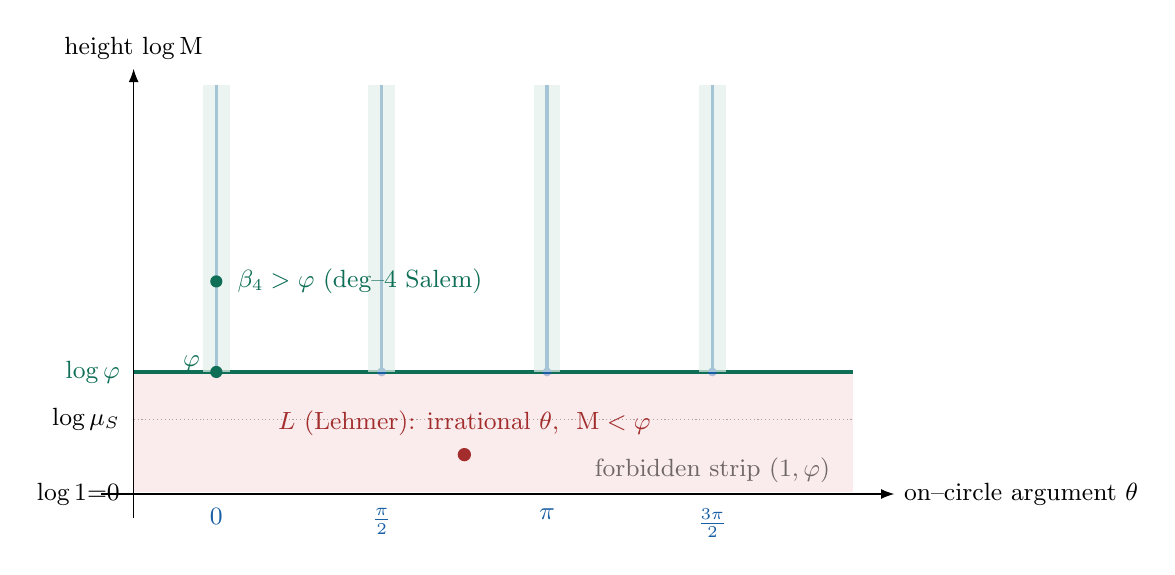
\begin{tikzpicture}[x=1.05cm,y=1.0cm,>=Latex]
% axes
\draw[->] (-0.4,0) -- (9.2,0) node[right]{\small on--circle argument $\theta$};
\draw[->] (0,-0.3) -- (0,5.4) node[above]{\small height $\log\Mah$};
% baseline M=1
\draw[dashed] (0,0.0) -- (8.7,0.0);
\node[left] at (-0.05,0.0) {\small $\log1{=}0$};
% floor line at log phi
\draw[forcedc,very thick] (0,1.55) -- (8.7,1.55);
\node[left,forcedc] at (-0.05,1.55) {\small $\log\varphi$};
% mu_S marker
\draw[densely dotted] (0,0.95) -- (8.7,0.95);
\node[left] at (-0.05,0.95) {\small $\log\mu_S$};
% lattice posts at 0, pi/2, pi, 3pi/2 -> x = 0.0(real axis shown at 1.0), 3.0, 5.0, 7.0
\foreach \x/\lab in {1.0/$0$,3.0/$\frac\pi2$,5.0/$\pi$,7.0/$\frac{3\pi}2$}{
  \draw[declaredc,very thick] (\x,1.55) -- (\x,5.2);
  \node[below,declaredc] at (\x,-0.06) {\small \lab};
  \fill[declaredc] (\x,1.55) circle (1.6pt);
}
% shaded box region: above floor, at the four posts (illustrate as faint columns)
\foreach \x in {1.0,3.0,5.0,7.0}{
  \fill[boxfill,opacity=0.7] (\x-0.16,1.55) rectangle (\x+0.16,5.2);
}
% forbidden strip (1,phi)
\fill[forbidfill,opacity=0.7] (0,0.02) rectangle (8.7,1.53);
\node[forbidfill!45!black] at (7.0,0.30) {\small forbidden strip $(1,\varphi)$};
% phi on the floor at the theta=0 post (labelled to its left)
\fill[forcedc] (1.0,1.55) circle (2.2pt);
\node[forcedc,anchor=east] at (0.92,1.66) {\small $\varphi$};
% beta4 above the floor at the theta=0 post (minimal degree-4 Salem)
\fill[forcedc] (1.0,2.70) circle (2.2pt);
\node[forcedc,anchor=west] at (1.14,2.70) {\small $\beta_4>\varphi$ (deg--4 Salem)};
% Lehmer: irrational angle (between posts), below the floor and below mu_S -> OUTSIDE
\fill[openc] (4.0,0.50) circle (2.4pt);
\node[openc,anchor=south] at (4.0,0.62) {\small $L$ (Lehmer): irrational $\theta$,\ \ $\Mah<\varphi$};
\end{tikzpicture}
\caption{\small Lehmer's Box (shaded columns). The \textcolor{forcedc}{green floor wall} is $\log\varphi$; the \textcolor{declaredc}{blue lattice walls} are the four on--circle directions $\tfrac\pi2\Z$. An emitted on--circle eigenvalue must sit on a blue post \emph{and} above the green floor. The golden seed $\varphi$ realises the floor; the minimal degree--four Salem $\beta_4$ sits above it. Lehmer's number $L$ lies \textcolor{openc}{outside the box on both counts}: its on--circle conjugates carry irrational angle (between the posts) and its measure lies in the forbidden strip below $\varphi$. The box excludes it as an \emph{emission}; it does nothing to it as a \emph{number}.}
\label{fig:box}
\end{figure}

\begin{theorem}[Emission $\subseteq$ Box]\label{thm:emitbox}
Every matrix in the spectral emission algebra $\Scal$ lies in Lehmer's Box: $\Scal\subseteq\Box$. \forced{} {\small(assembles \texttt{P2-ANG-01..03}, \texttt{P2-GAP-02})}
\end{theorem}
\begin{proof}
Floor wall: by Lemma~\ref{lem:base} every catalog measure is in $\{1\}\cup[\varphi,\infty)$, and by Lemma~\ref{lem:degraise} the spectral operators preserve membership in $\{1\}\cup[\varphi,\infty)$; hence every emitted measure avoids $(1,\varphi)$. Lattice walls: by Lemma~\ref{lem:catargs} every catalog eigenvalue has argument in $\tfrac\pi2\Z$, and by Lemma~\ref{lem:closure} the operators preserve this; hence every emitted on--circle eigenvalue has argument in $\tfrac\pi2\Z$, i.e.\ lies in $\mu_4$. Both defining conditions of \eqref{eq:box} hold for every element of $\Scal$.
\end{proof}

\begin{theorem}[Salem $\cap$ Box $=\varnothing$]\label{thm:salemoutside}
No Salem number's minimal polynomial lies in Lehmer's Box. \forced{} {\small(\texttt{P2-ANG-04}, \texttt{P2-ANG-05})}
\end{theorem}
\begin{proof}
Let $\beta$ be a Salem number. Its degree is $2m\ge4$, so $m_\beta$ has at least one on--circle conjugate $\zeta$ (Definition~\ref{def:pisotsalem}). By Lemma~\ref{lem:salemirr}, $\arg\zeta\notin\tfrac\pi2\Z$, so $\arg\zeta\in\argc(m_\beta)$ violates the lattice--wall condition of \eqref{eq:box}. Hence $m_\beta\notin\Box$. (The floor wall is also violated whenever $\Mah(\beta)<\varphi$, as for $\beta=L$; a single violated wall already places $m_\beta$ outside the box.)
\end{proof}

\begin{corollary}[Exclusion and the positive floor]\label{cor:floor}
The emission image contains no Salem number; consequently $\Mah(\Scal)\subseteq\{1\}\cup[\mu_S,\infty)$, realised at $\varphi$, and for every emittable $\theta$ with $\Mah(\theta)>1$,
\begin{equation}\label{eq:floorval}
\lambda\log\Mah(\theta)\ \ge\ \lambda\log\mu_S\ >\ 0,\qquad \log\mu_S=0.281200\ldots,\ \ \text{realised at}\ \log\varphi=0.481212\ldots\ \text{nats}.
\end{equation}
\forced{} {\small(\texttt{P2-GAP-03}, \texttt{P2-EALG-06})}
\end{corollary}
\begin{proof}
Suppose a Salem $\beta$ were emitted: some $M\in\Scal$ has $m_\beta\mid\charp_M$, so $M\in\Box$ by Theorem~\ref{thm:emitbox}, forcing $m_\beta\in\Box$ --- contradicting Theorem~\ref{thm:salemoutside}. Hence no Salem is emitted. Every measure in $(1,\mu_S)$ is realised only by a reciprocal Salem--type number (non--reciprocals obey Smyth, Lemma~\ref{lem:smyth}); with the Salem locus excluded, $\Mah(\Scal)$ omits $(1,\mu_S)$, giving \eqref{eq:floorval}. The realised minimum is $\varphi$ by Lemma~\ref{lem:degraise}. The exchange rate $\lambda=2c$ is linear in the free conformal constant $c$, so the floor $2c\log\varphi$ scales with $c$ and never collapses to $0$.
\end{proof}

This is the whole mechanism. The remaining sections give the box three further faces and close the one operator the spectral argument does not reach.

\section{The signature face: where a real Salem could graze the floor}\label{sec:sigface}

The lattice walls are an \emph{angular} statement; there is an equivalent \emph{field--theoretic} statement that locates precisely the one place a real Salem number could approach the floor and shows the floor survives there too.

\begin{proposition}[Salem forces a Lorentzian signature]\label{prop:lorentz}
A Salem field of degree $2m$ has unit--rank signature $(r_1,r_2)=(2,m-1)$ and trace--form signature $(m+1,m-1)$, indefinite for $m\ge2$. A number is Salem only if its field carries a complex embedding \emph{on} the unit circle. \forced{} {\small(\texttt{P2-NL-02}, \texttt{P2-NL-03})}
\end{proposition}
\begin{proof}
The two real embeddings send $\beta\mapsto\beta,\beta^{-1}$; the remaining $m-1$ conjugate pairs are the on--circle conjugates, giving $(r_1,r_2)=(2,m-1)$ and trace--form signature $(r_1+r_2,\,r_2)=(m+1,m-1)$. ``On the circle'' is the defining condition for the complex places.
\end{proof}

So a Salem number needs a degree--$\ge4$ field of signature $(2,m-1)$. The construction's real spectral data live in a single, fully enumerable field, and almost none of its subfields have that shape.

\begin{lemma}[Real differences are field--confined]\label{lem:diffconf}
The real differences of catalog eigenvalues lie in $K=\Q(\sqrt2,\sqrt3,5^{1/4})$, of degree $16$. \forced{} {\small(\texttt{P2-UNIF-02})}
\end{lemma}
\begin{proof}
The real catalog eigenvalues are rational combinations of $\sqrt2,\sqrt3,\sqrt5,\varphi=\tfrac{1+\sqrt5}2$, and the real root $5^{1/4}/\varphi$ of $K$; all lie in $K$, and $K$ is closed under subtraction. The composite degree is $[\Q(\sqrt2):\Q]\,[\Q(\sqrt3):\Q]\,[\Q(5^{1/4}):\Q]=2\cdot2\cdot4=16$.
\end{proof}

\begin{theorem}[Signature lattice of $K$, exhaustive]\label{thm:siglattice}
Every one of the $27$ subfields of $K$ is either totally real ($r_2=0$) or of signature $(2k,k)$ for some $k\ge1$; the Salem shape $(2,1)$ occurs for exactly four quartic subfields, and $K$ itself has signature $(8,4)$. The full census, by $(\deg,r_1,r_2)$, is
\[
\begin{array}{c|ccccccc}
(\deg,r_1,r_2) & (1,1,0) & (2,2,0) & (4,2,1) & (4,4,0) & (8,4,2) & (8,8,0) & (16,8,4)\\\hline
\#\ \text{subfields} & 1 & 7 & 4 & 7 & 6 & 1 & 1
\end{array}
\]
totalling $27$. \computed{} {\small(\texttt{P2-UNIF-03}; Galois correspondence on the closure $K(i)$, $G\cong C_2\times C_2\times D_4$, all $27$ subgroups enumerated)}
\end{theorem}

The structural content extracted from the census is what the floor needs:

\begin{corollary}[Degree--four Salem floor]\label{cor:deg4}
The only Salem--bearing subfields of $K$ are the four quartic fields of signature $(2,1)$. The minimal degree--four Salem number is
\[
\beta_4\ =\ 1.7220838057\ldots,\qquad m_{\beta_4}(x)=x^4-x^3-x^2-x+1,\qquad \beta_4>\varphi,
\]
so every Salem number realisable in $K$ has $\Mah\ge\beta_4>\varphi$. The image meets no sub--$\varphi$ Salem: $\operatorname{image}(\Scal)\cap\{\text{Salem}:\Mah<\varphi\}=\varnothing$. \forced{} {\small(\texttt{P2-UNIF-04}, \texttt{P2-UNIF-05})}
\end{corollary}
\begin{proof}
A Salem field has signature $(2,m-1)$ (Proposition~\ref{prop:lorentz}); among the subfields of $K$ the only signatures of the form $(2,m-1)$ are the four $(2,1)$ quartics (Theorem~\ref{thm:siglattice}), forcing degree four. The minimal Mahler measure among degree--four Salem numbers is attained by $x^4-x^3-x^2-x+1$, whose dominant root $\beta_4=1.7221\ldots$ exceeds $\varphi=1.6180\ldots$ --- decided exactly, since $\beta_4>\varphi\iff m_{\beta_4}(\varphi)<0$, and $m_{\beta_4}(\varphi)=\varphi^4-\varphi^3-\varphi^2-\varphi+1$ evaluates in $\Q(\sqrt5)$ to a negative element by the sign rule of Section~\ref{sec:door}. Hence no emitted Salem lies below $\varphi$.
\end{proof}

The signature face is the geometric face of the lattice walls: a Salem number needs an on--circle complex place; the construction's only indefinite (Lorentzian) field is the quartic $\Q(5^{1/4})$, whose complex place sits \emph{off} the circle ($\abs{i\beta}=2.4195$, $\abs{5^{1/4}i}=1.4953$), and the spectral operators --- which only multiply, union, double, and preserve spectra --- cannot rotate it onto the circle without producing a rational angle, i.e.\ a fourth root of unity, not a Salem conjugate. The gate's discriminant flip $D=t^2-4$ reappears here as the field's signature split.

\section{The trace--down face: the box boundary as the \texorpdfstring{$t=2$}{t=2} flip}\label{sec:flipface}

A fourth face relocates the entire Salem question to a single decidable boundary, which the spectral operators are shown never to cross. This is the face that will let us handle the entry--level operators in Section~\ref{sec:door}.

\begin{definition}[Trace--down]\label{def:tracedown}
For a reciprocal $m_\theta$ of degree $2m$, the substitution $t=\theta+\theta^{-1}$ yields a degree--$m$ polynomial $T$, the \emph{trace--down}: $m_\theta(x)=x^m\,T(x+x^{-1})$.
\end{definition}

\begin{lemma}[Salem $=$ flip--straddle]\label{lem:salemflip}
A reciprocal integer $\theta$ is a Salem number if and only if its trace--down $T$ is totally real with exactly one root in $(2,\infty)$ and the remaining $m-1$ roots in $(-2,2)$. \forced{} {\small(\texttt{P2-DELTA-02})}
\end{lemma}
\begin{proof}
Under $t=\theta+\theta^{-1}$ a reciprocal pair $\{\theta,\theta^{-1}\}$ maps to a single $t$. A pair on the unit circle, $\theta=e^{i\psi}$, gives $t=2\cos\psi\in(-2,2)$ (real, inside); a real pair with $\theta>1$ gives $t=\theta+\theta^{-1}>2$. Thus the Salem condition --- exactly one reciprocal pair off the circle (the dominant $\beta,\beta^{-1}$) and all others on it --- is precisely one trace--down root past $+2$ and the rest inside $(-2,2)$. The boundary $t=\pm2$ corresponds to $\theta=\pm1$, where the discriminant of $x^2-tx+1$ is $D=t^2-4$ changing sign: $D>0$ off the circle, $D<0$ on it. This is the $\lambda=2c$ flip.
\end{proof}

\begin{proposition}[Spectral operators sit at the flip, never astride it]\label{prop:specflip}
For every spectral operator, each emitted reciprocal factor has a trace--down that is totally real and does \emph{not} straddle $t=2$ in the Salem pattern: its off--circle roots come in the cyclotomic ($t=\pm2$, $D=0$) or totally real configurations, never the single--straddle of Lemma~\ref{lem:salemflip}. \forced{} {\small(\texttt{P2-DELTA-01}, \texttt{P2-DELTA-04})}
\end{proposition}
\begin{proof}
By Theorem~\ref{thm:emitbox} an emitted on--circle eigenvalue is a fourth root of unity, whose trace--down value is $t\in\{2,0,-2\}$ --- the cyclotomic lattice $\{2,0,-2\}=\{\rho(1),\rho(\pm i),\rho(-1)\}$ under $\rho(z)=z+z^{-1}$. A genuine Salem straddle requires an on--circle pair at irrational angle, i.e.\ $t\in(-2,2)$ irrational and not in $\{0\}$, which the lattice walls forbid. Hence no emitted trace--down exhibits the Salem straddle.
\end{proof}

\section{The one door: the free commutator and the lock}\label{sec:door}

Theorem~\ref{thm:emitbox} confines the \emph{spectral} algebra to the box because every spectral operator's effect on the spectrum is forced. The entry--level operators are different: their characteristic polynomials are not determined by the inputs' spectra, so the angle argument does not directly apply. We dispose of them by relocating each to the trace--down boundary of Section~\ref{sec:flipface}, and we treat the hardest --- the commutator --- both structurally and operationally.

\subsection{The circulant is forced outright}
\begin{proposition}[Cyclotomic obstruction]\label{prop:circ}
No integer circulant emits a Salem number. \forced{} {\small(\texttt{P2-CIRC-01})}
\end{proposition}
\begin{proof}
The eigenvalues of $\operatorname{circ}(c_0,\dots,c_{n-1})$ are $\lambda_j=\sum_k c_k\omega^{jk}$ with $\omega=e^{2\pi i/n}$, all in the cyclotomic field $\Q(\zeta_n)$, which is abelian over $\Q$ and therefore totally real or CM. A Salem field has signature $(2,m-1)$ with $m\ge2$: two real embeddings (not totally complex) and a complex pair (not totally real), hence not abelian. So no circulant eigenvalue can be a Salem number; equivalently a real Salem eigenvalue would force its on--circle conjugates real, a contradiction.
\end{proof}

\subsection{Shoda's theorem: the commutator is the door}
\begin{lemma}[Shoda; Albert--Muckenhoupt; Laffey--Reams]\label{lem:shoda}
Over a field, a square matrix is a commutator $[X,Y]=XY-YX$ if and only if it has trace zero
\cite{Shoda1936}; over $\Z$, every trace--zero integer matrix is an integer commutator
\cite{AlbertMuckenhoupt,LaffeyReams}. \forced{}
\end{lemma}

Lemma~\ref{lem:shoda} is exactly why the commutator is dangerous: the only constraint on $[A,B]$ is tracelessness, so a free commutator can realise \emph{any} traceless integer matrix --- including one whose characteristic polynomial carries Lehmer's degree--ten sub--$\varphi$ Salem. No a priori field or angle constraint survives. The free commutator is the single field--breaking operation, the one door out of the box.

\subsection{Structural closure: the framework's commutator is a derivation}
The construction does not use a free commutator. Its commutator is the \emph{self--action}.

\begin{definition}[Self--action]\label{def:selfaction}
For a seed companion $R$, the self--action is $\ad_R=[R,\cdot]:X\mapsto RX-XR$, a derivation on the matrix algebra.
\end{definition}

\begin{lemma}[Difference spectrum]\label{lem:diffspec}
The spectrum of $\ad_R$ is the difference set $\{\lambda_i-\lambda_j\}$ of the eigenvalues of $R$. For the golden seed, $\spec(\ad_R)=\{0,+\sqrt5,-\sqrt5\}$. \forced{} {\small(\texttt{P2-UNIF-01})}
\end{lemma}
\begin{proof}
A derivation $\ad_R$ acts on the rank--one matrices $E_{ij}=v_i w_j^{\!\top}$ (with $v_i,w_j$ the right/left eigenvectors of $R$) by $\ad_R E_{ij}=(\lambda_i-\lambda_j)E_{ij}$, so its eigenvalues are exactly the pairwise differences. For $R=C(x^2-x-1)$ with eigenvalues $\varphi,\psi=-\varphi^{-1}$, the differences are $0$ and $\pm(\varphi-\psi)=\pm\sqrt5$.
\end{proof}

Because $\ad_R$ is a derivation, its spectrum is \emph{forced} to be the eigenvalue difference set; its real eigenvalues are differences of catalog eigenvalues, which lie in $K$ by Lemma~\ref{lem:diffconf}. By the signature lattice (Theorem~\ref{thm:siglattice}) every subfield of $K$ is totally real or $(2k,k)$, and the only Salem--bearing subfield carries $\Mah\ge\beta_4>\varphi$ (Corollary~\ref{cor:deg4}). Hence:

\begin{theorem}[Uniform self--action bound]\label{thm:uniform}
The self--action commutator keeps every emitted measure in $\{1\}\cup[\varphi,\infty)$ at \emph{every} size: the floor $\log\varphi$ is forced uniformly, not checked instance by instance. \forced{} {\small(\texttt{P2-UNIF-01..05})}
\end{theorem}

This upgrades the floor from a per--instance check to a uniform bound for the framework's actual commutator, by using the structure the algebra is derived from rather than extending the angle argument.

\subsection{Operational lock: the exact closure guard}
For the residual case --- a \emph{free}, non--self--action commutator at unbounded size --- the Salem question is the Sturm--decidable flip--straddle of Lemma~\ref{lem:salemflip}, and the floor is certified at runtime by an exact guard.

\begin{proposition}[Closure guard]\label{prop:guard}
There is a function $\textsf{validate}(M)$ returning one of three verdicts, decided in exact arithmetic:
\[
\textsf{FORCED}\ (\text{no Salem factor}),\quad
\textsf{FORCED\_ABOVE\_FLOOR}\ (\text{Salem factor, but }\beta\ge\varphi),\quad
\textsf{INVALID\_CLOSURE}\ (\text{a Salem factor with }\beta<\varphi).
\]
The decision $\beta<\varphi$ is made by the sign of $m_\beta(\varphi)$ in $\Q(\sqrt5)$, with no floating point. Framework objects read \textsf{FORCED}; a planted minimal degree--four Salem $\beta_4$ reads \textsf{FORCED\_ABOVE\_FLOOR}; a foreign traceless carrier of Lehmer's number reads \textsf{INVALID\_CLOSURE}. \forced{} {\small(\texttt{P2-GUARD-01..05})}
\end{proposition}
\begin{proof}[Mechanism]
Write a candidate test value as $a+b\sqrt5$ with $a,b\in\Q$. Its sign is decided exactly: if $a,b$ share a sign the sign is theirs; otherwise compare $a^2$ against $5b^2$ as integers (after clearing denominators), which decides $a+b\sqrt5\gtrless0$ with no irrational evaluation. Applying this to $m_\beta(\varphi)$ decides $\beta\gtrless\varphi$ on the exact boundary. The verdict ladder is then: no reciprocal degree--$\ge4$ factor $\Rightarrow$ \textsf{FORCED}; such a factor with $m_\beta(\varphi)\le0$ (i.e.\ $\beta\ge\varphi$) $\Rightarrow$ \textsf{FORCED\_ABOVE\_FLOOR}; with $m_\beta(\varphi)>0$ (i.e.\ $\beta<\varphi$) $\Rightarrow$ \textsf{INVALID\_CLOSURE}.
\end{proof}

\begin{remark}[The guard is the floor certificate, not the no--Salem theorem]\label{rem:guardscope}
The guard returns \textsf{INVALID\_CLOSURE} only for a \emph{sub--$\varphi$} Salem; it permits \textsf{FORCED\_ABOVE\_FLOOR}. It is therefore the exact runtime \emph{certificate of the cost floor} --- complementary to, not a replacement for, the angle theorem (Theorem~\ref{thm:salemoutside}), which excludes \emph{every} Salem from the spectral image. ``Floor holds'' (guard) and ``no Salem emitted'' (angle theorem) are distinct statements and are not conflated.
\end{remark}

\section{The sidestep, stated precisely}\label{sec:sidestep}

We now make exact the relationship between the box theorem and Lehmer's problem. Three statements:
\begin{align}
\textbf{(P)}\quad & \inf\{\Mah(p):p\in\Z[x],\ \Mah(p)>1\}>1\qquad\text{(Lehmer's problem; open).}\notag\\
\textbf{(C)}\quad & \text{that infimum equals }\Mah(L)=1.17628\ldots\qquad\text{(Lehmer's conjecture; open, stronger).}\notag\\
\textbf{(B)}\quad & \Scal\subseteq\Box\ \Rightarrow\ \Mah(\Scal)\subseteq\{1\}\cup[\mu_S,\infty),\ \text{realised at }\varphi\qquad\text{(this paper; proved).}\notag
\end{align}

\begin{proposition}[Logical position of the box theorem]\label{prop:logic}
\emph{(i)} \textbf{(C)} implies the floor that \textbf{(B)} asserts for $\Scal$; thus \textbf{(B)} is logically weaker than \textbf{(C)}, and far narrower in scope ($\Scal$ versus all of $\Z[x]$). \emph{(ii)} \textbf{(B)} does not imply \textbf{(P)}: it says nothing about Salem numbers outside $\Scal$. \emph{(iii)} \textbf{(B)} is unconditional --- its proof assumes neither \textbf{(P)} nor \textbf{(C)}. \emph{(iv)} \textbf{(B)} is consistent with both truth values of \textbf{(P)}.
\end{proposition}
\begin{proof}
(i) If the global infimum exceeds $1$, then \emph{a fortiori} the infimum over the subset of emittable directions exceeds $1$; so \textbf{(C)} (hence \textbf{(P)}) gives \textbf{(B)}'s floor immediately. The converse fails by (ii). (ii) Lehmer's number $L$ is a Salem number that exists independently of the construction; Theorems~\ref{thm:emitbox}--\ref{thm:salemoutside} place $m_L$ \emph{outside} the box and therefore exclude $L$ from $\Scal$, but they assert nothing about the value of $\Mah(L)$ or about Salem numbers in general. (iii) The proof of \textbf{(B)} uses only Lemmas~\ref{lem:base}--\ref{lem:salemirr} and the closure of the operators, none of which presupposes a global height bound. (iv) Suppose \textbf{(P)} is false, i.e.\ Salem numbers accumulate at $1$. Every such small Salem number violates a wall of the box (irrational on--circle angle, by Lemma~\ref{lem:salemirr}), hence is not emitted; \textbf{(B)} still holds. Suppose \textbf{(P)} is true; then \textbf{(B)} holds a fortiori. So \textbf{(B)} neither entails nor contradicts \textbf{(P)}.
\end{proof}

\begin{corollary}[The sidestep]\label{cor:sidestep}
The construction obtains the positive cost floor required by \eqref{eq:floorgoal} without deciding Lehmer's problem. It confines its own emissions to Lehmer's Box, from which the entire Salem locus --- and with it the whole open band $(1,\mu_S)$ --- is provably absent. Lehmer's number is excluded as an emission, never as a number; the open problem is left exactly where it stood.
\end{corollary}

\begin{remark}[What is genuinely open, and what only looked open]\label{rem:residue}
Two fronts, of different kinds. \emph{(a)} The \emph{free} (non--self--action) commutator is the one door (Lemma~\ref{lem:shoda}). It is closed structurally where it is the framework's self--action (Theorem~\ref{thm:uniform}) and per instance by the Sturm--decidable flip--straddle (Lemma~\ref{lem:salemflip}) and the exact guard (Proposition~\ref{prop:guard}). What is \emph{not} available is a single uniform theorem asserting a floor or gap over \emph{every} free commutator at all sizes --- and this is not an open gap awaiting a proof but an \textbf{unsatisfiable} target. By Lemma~\ref{lem:shoda} the trace--zero integer companion carrying Lehmer's number \emph{is} a commutator, and it sits at $\Mah(L)=1.17628\ldots<\varphi$; so any uniform floor/gap statement over all free commutators is \emph{false} on that one witness --- refuted by construction, not open. There is accordingly no such theorem to prove, and the box closure is consequently \textbf{operation--relative}: it holds on the spectral emission algebra $\Scal$, whose operations force the spectrum, \emph{not} on the ambient algebra $\Acal$ where Shoda's commutators live. The underlying Shoda fact is \forced{}; the only residue --- deciding a \emph{given} free commutator --- is discharged exactly by the guard (Proposition~\ref{prop:guard}), per instance. \emph{(b)} Lehmer's problem \textbf{(P)} itself remains genuinely open in number theory, untouched. \openq{} The first front only looked open; the second is named and left exactly where it stood.
\end{remark}

\section{Epistemic ledger}\label{sec:ledger}

Each load--bearing claim, its status, and the machine--verified test that backs it. Statuses follow the companion suite's discipline: \forced{}/\computed{} are asserted and proved here \emph{and} re--derived in exact arithmetic; \declared{}/\openq{} are modelling choices or named open fronts, recorded as context.

\begin{center}
\renewcommand{\arraystretch}{1.18}
\begin{tabular}{@{}p{6.6cm}cl@{}}
\toprule
\textbf{Claim} & \textbf{Status} & \textbf{Backing test} \\
\midrule
Empty quadratic strip $(1,\varphi)$; minimiser $\varphi$ at disc $5$ & \forced & \texttt{P1-GATE-02/03} \\
Operators preserve the floor; image $\subseteq\{1\}\cup[\varphi,\infty)$ & \forced & \texttt{P2-EALG-01/02} \\
Catalog arguments in $\tfrac\pi2\Z$ & \forced & \texttt{P2-ANG-01} \\
$\tfrac\pi2\Z$ closed under $+$ and doubling, not halving & \forced & \texttt{P2-ANG-02} \\
On--circle $+$ arg in $\tfrac\pi2\Z$ $\Rightarrow$ fourth root of unity & \forced & \texttt{P2-ANG-03} \\
Salem on--circle conjugates are not roots of unity & \forced & \texttt{P2-ANG-04} \\
No Salem emitted (Box exclusion) & \forced & \texttt{P2-ANG-05} \\
Positive cost floor $2c\log\varphi$, linear in free $c$ & \forced & \texttt{P2-GAP-03}, \texttt{P2-EALG-06} \\
Salem field signature $(2,m-1)$, Lorentzian & \forced & \texttt{P2-NL-02/03} \\
$27$--subfield signature lattice; four $(2,1)$ quartics & \computed & \texttt{P2-UNIF-03} \\
Minimal degree--four Salem $\beta_4>\varphi$; image $\cap$ sub--$\varphi$ Salem $=\varnothing$ & \forced & \texttt{P2-UNIF-04/05} \\
Self--action difference spectrum $\{0,\pm\sqrt5\}$; uniform floor & \forced & \texttt{P2-UNIF-01} \\
Trace--down: Salem $\iff$ flip--straddle at $t=2$ & \forced & \texttt{P2-DELTA-02} \\
Circulant emits no Salem (cyclotomic/CM) & \forced & \texttt{P2-CIRC-01} \\
Closure guard ladder; $\beta<\varphi$ by sign in $\Q(\sqrt5)$ & \forced & \texttt{P2-GUARD-01..05} \\
Shoda: trace zero $\Rightarrow$ commutator; Lehmer carrier is one, $<\varphi$ & \forced & Lem~\ref{lem:shoda}; \texttt{P2-GUARD-05} \\
Uniform theorem over \emph{every} free commutator: unsatisfiable; closure operation--relative & \forced & \texttt{P2-GUARD-01..05} \\
Conformal constant $c$ (Jeffreys reading $c=1$) & \declared & --- \\
Lehmer's problem \textbf{(P)} itself (number theory) & \openq & --- \\
\bottomrule
\end{tabular}
\end{center}

\paragraph{Closing statement.} Lehmer's Box is not a new theorem so much as a new \emph{shape} for an old one: the floor wall $\varphi$ and the lattice walls $\tfrac\pi2\Z$ are the height and angle faces of a single confinement, with the field signature and the trace--down flip as its other two faces. The construction stays inside the box because every spectral operation respects both walls, and the one operation that could leave --- the free commutator --- is closed structurally where it is the self--action and locked operationally where it is not. Salem numbers, Lehmer's among them, live outside the box. We have not shown they cannot come close to $1$; we have shown the construction never goes to fetch them. That is the precise sense in which this work sidesteps Lehmer's problem without disproving it.

\begin{thebibliography}{9}
\bibitem{Lehmer} D.~H.~Lehmer, \emph{Factorization of certain cyclotomic functions}, Annals of Mathematics (2) \textbf{34} (1933), 461--479.
\bibitem{Smyth} C.~J.~Smyth, \emph{On the product of the conjugates outside the unit circle of an algebraic integer}, Bulletin of the London Mathematical Society \textbf{3} (1971), 169--175.
\bibitem{Dobrowolski} E.~Dobrowolski, \emph{On a question of Lehmer and the number of irreducible factors of a polynomial}, Acta Arithmetica \textbf{34} (1979), 391--401.
\bibitem{Salem} R.~Salem, \emph{Power series with integral coefficients}, Duke Mathematical Journal \textbf{12} (1945), 153--172.
\bibitem{LSW} D.~Lind, K.~Schmidt, T.~Ward, \emph{Mahler measure and entropy for commuting automorphisms of compact groups}, Inventiones Mathematicae \textbf{101} (1990), 593--629.
\bibitem{Shoda1936} K.~Shoda, \emph{Einige S\"atze \"uber Matrizen}, Japanese Journal of Mathematics \textbf{13} (1936), 361--365. [Bibliographic details unverified --- see provenance note.]
\bibitem{AlbertMuckenhoupt} A.~A.~Albert and B.~Muckenhoupt, \emph{On matrices of trace zero}, Michigan Mathematical Journal \textbf{4} (1957), 1--3. [Bibliographic details unverified --- see provenance note.]
\bibitem{LaffeyReams} T.~J.~Laffey and R.~Reams, \emph{Integral similarity and commutators of integral matrices}, Linear Algebra and its Applications \textbf{197--198} (1994), 671--689. [Bibliographic details unverified --- see provenance note.]
\end{thebibliography}

\smallskip
\noindent\footnotesize\emph{Provenance caveat.} The commutator references (Shoda 1936; Albert--Muckenhoupt 1957; Laffey--Reams 1994), which back Lemma~\ref{lem:shoda} and the operation--relative closure of Remark~\ref{rem:residue}, are standard attributions supplied from memory; their volume/page/year details have \emph{not} been machine--verified and should be checked against the primary sources before external use. The Lehmer, Smyth, Dobrowolski, Salem, and LSW citations are likewise standard attributions recorded for orientation.

\end{document}
